\begin{figure}[ht]
  \centering
  \begin{subfigure}[b]{0.48\textwidth}
    \centering
    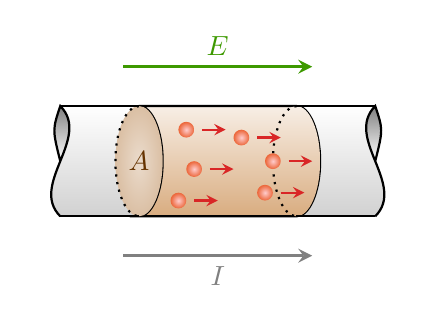
\begin{tikzpicture}[>=stealth]
      \def\rx{0.3}
      \def\ry{0.7}
      \def\lle{1}
      \def\cond{1}
      \def\curv{0.4}
      
      % Sombra conductor
      \shade[top color=orange!70!black!10, bottom color=orange!70!black!50] 
        (-\lle, \ry) -- (\lle, \ry)
        arc (90:-90:\rx cm and \ry cm)
        -- (-\lle, -\ry)
        arc (-90:90:\rx cm and \ry cm);

      % Sombra D (de corte)
      \shade (-\lle-\cond,0) .. controls (-\lle-\cond+\curv, 0.3) .. (-\lle-\cond, \ry) .. controls (-\lle-\cond-\curv+0.3, 0.4) .. (-\lle-\cond, 0);
      \shade (\lle+\cond,0) .. controls (\lle+\cond-\curv, 0.3) .. (\lle+\cond, \ry) .. controls (\lle+\cond+\curv-0.3, 0.4) .. (\lle+\cond, 0);

      % Sombra corte
      \shade[top color=white, bottom color=white!70!black!60] 
        (-\lle,-\ry) -- (-\lle-\cond,-\ry) .. controls (-\lle-\cond-\curv, -0.3) and (-\lle-\cond+\curv, 0.3) .. (-\lle-\cond, \ry) -- (-\lle,\ry);
      \shade[top color=white, bottom color=white!70!black!60] 
        (\lle,-\ry) -- (\lle+\cond,-\ry) .. controls (\lle+\cond+\curv, -0.3) and (\lle+\cond-\curv, 0.3) .. (\lle+\cond, \ry) -- (\lle,\ry);

      \draw[thick] 
        (-\lle, \ry) -- (\lle, \ry)
        arc (90:-90:\rx cm and \ry cm)
        -- (-\lle, -\ry)
        arc (-90:90:\rx cm and \ry cm);


      \shade[bottom color=orange!70!black!50, top color=orange!70!black!10] (\lle,0) ellipse (\rx cm and \ry cm);
      \shade[outer color=orange!60!black!36, inner color=orange!60!black!20] (-\lle,0) ellipse (\rx cm and \ry cm);

      % Sección de corte
      \draw[black,thick] (-\lle-\cond,-\ry) .. controls (-\lle-\cond-\curv, -0.3) and (-\lle-\cond+\curv, 0.3) .. (-\lle-\cond, \ry) .. controls (-\lle-\cond-\curv+0.3, 0.4) .. (-\lle-\cond, 0);
      \draw[black,thick] (\lle+\cond,-\ry) .. controls (\lle+\cond+\curv, -0.3) and (\lle+\cond-\curv, 0.3) .. (+\lle+\cond, \ry) .. controls (\lle+\cond+\curv-0.3, 0.4) .. (\lle+\cond, 0);
      \draw[black,thick] (-\lle,\ry) -- (-\lle-\cond,\ry);
      \draw[black,thick] (-\lle,-\ry) -- (-\lle-\cond,-\ry);
      \draw[black,thick] (\lle,\ry) -- (\lle+\cond,\ry);
      \draw[black,thick] (\lle,-\ry) -- (\lle+\cond,-\ry);

      \draw[thick, dotted] (-\lle,\ry) arc (90:270:\rx cm and \ry cm);
      \draw[thick, dotted] (\lle,\ry) arc (90:270:\rx cm and \ry cm);

      \node at (-\lle, 0) {\color{orange!40!black}\(A\)};

      % Dirección de la corriente convencional
      \draw[very thick, gray, ->] (-\lle-0.2,-\ry-0.5) -- node[below]{\(I\)} (\lle+0.2,-\ry-0.5);
      % Dirección del campo eléctrico
      \draw[very thick, green!60!yellow!60!black, ->] (-\lle-0.2,\ry+0.5) -- node[above]{\(E\)} (\lle+0.2,\ry+0.5);

      % Cargas
      \foreach \x\y in {-0.4/0.4,-0.3/-0.1,-0.5/-0.5,0.3/0.3,0.7/0,0.6/-0.4} {
        \shade[inner color=white!80!red, outer color=orange!50!red!70!lightgray] (\x,\y) circle (.1) [radius=1pt];
        \draw[thick,color=red!70!gray,->] (\x+0.2,\y) -- (\x+0.5,\y) ;
      }
    \end{tikzpicture}
    \caption{Una corriente convencional es tratada como un flujo de cargas positivas, sin importar si las cargas libres del conductor son positivas, negativas o ambas.}
    \label{fig:flujo_de_cargas_positivas}
  \end{subfigure}
  \hfill
  \begin{subfigure}[b]{0.48\textwidth}
    \centering
    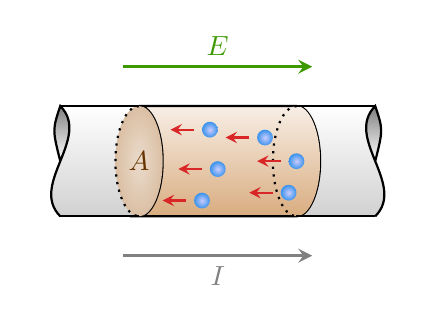
\begin{tikzpicture}[>=stealth]
      \def\rx{0.3}
      \def\ry{0.7}
      \def\lle{1}
      \def\cond{1}
      \def\curv{0.4}
      
      % Sombra conductor
      \shade[top color=orange!70!black!10, bottom color=orange!70!black!50] 
        (-\lle, \ry) -- (\lle, \ry)
        arc (90:-90:\rx cm and \ry cm)
        -- (-\lle, -\ry)
        arc (-90:90:\rx cm and \ry cm);

      % Sombra D (de corte)
      \shade (-\lle-\cond,0) .. controls (-\lle-\cond+\curv, 0.3) .. (-\lle-\cond, \ry) .. controls (-\lle-\cond-\curv+0.3, 0.4) .. (-\lle-\cond, 0);
      \shade (\lle+\cond,0) .. controls (\lle+\cond-\curv, 0.3) .. (\lle+\cond, \ry) .. controls (\lle+\cond+\curv-0.3, 0.4) .. (\lle+\cond, 0);

      % Sombra corte
      \shade[top color=white, bottom color=white!70!black!60] 
        (-\lle,-\ry) -- (-\lle-\cond,-\ry) .. controls (-\lle-\cond-\curv, -0.3) and (-\lle-\cond+\curv, 0.3) .. (-\lle-\cond, \ry) -- (-\lle,\ry);
      \shade[top color=white, bottom color=white!70!black!60] 
        (\lle,-\ry) -- (\lle+\cond,-\ry) .. controls (\lle+\cond+\curv, -0.3) and (\lle+\cond-\curv, 0.3) .. (\lle+\cond, \ry) -- (\lle,\ry);

      \draw[thick] 
        (-\lle, \ry) -- (\lle, \ry)
        arc (90:-90:\rx cm and \ry cm)
        -- (-\lle, -\ry)
        arc (-90:90:\rx cm and \ry cm);


      \shade[bottom color=orange!70!black!50, top color=orange!70!black!10] (\lle,0) ellipse (\rx cm and \ry cm);
      \shade[outer color=orange!60!black!36, inner color=orange!60!black!20] (-\lle,0) ellipse (\rx cm and \ry cm);

      % Sección de corte
      \draw[black,thick] (-\lle-\cond,-\ry) .. controls (-\lle-\cond-\curv, -0.3) and (-\lle-\cond+\curv, 0.3) .. (-\lle-\cond, \ry) .. controls (-\lle-\cond-\curv+0.3, 0.4) .. (-\lle-\cond, 0);
      \draw[black,thick] (\lle+\cond,-\ry) .. controls (\lle+\cond+\curv, -0.3) and (\lle+\cond-\curv, 0.3) .. (+\lle+\cond, \ry) .. controls (\lle+\cond+\curv-0.3, 0.4) .. (\lle+\cond, 0);
      \draw[black,thick] (-\lle,\ry) -- (-\lle-\cond,\ry);
      \draw[black,thick] (-\lle,-\ry) -- (-\lle-\cond,-\ry);
      \draw[black,thick] (\lle,\ry) -- (\lle+\cond,\ry);
      \draw[black,thick] (\lle,-\ry) -- (\lle+\cond,-\ry);

      \draw[thick, dotted] (-\lle,\ry) arc (90:270:\rx cm and \ry cm);
      \draw[thick, dotted] (\lle,\ry) arc (90:270:\rx cm and \ry cm);

      \node at (-\lle, 0) {\color{orange!40!black}\(A\)};

      % Dirección de la corriente convencional
      \draw[very thick, gray, ->] (-\lle-0.2,-\ry-0.5) -- node[below]{\(I\)} (\lle+0.2,-\ry-0.5);
      % Dirección del campo eléctrico
      \draw[very thick, green!60!yellow!60!black, ->] (-\lle-0.2,\ry+0.5) -- node[above]{\(E\)} (\lle+0.2,\ry+0.5);

      % Cargas
      \foreach \x\y in {-0.1/0.4,0/-0.1,-0.2/-0.5,0.6/0.3,1/0,0.9/-0.4} {
        \shade[inner color=white!80!blue, outer color=cyan!50!blue!70!lightgray] (\x,\y) circle (.1) [radius=1pt];
        \draw[thick,color=red!70!gray,->] (\x-0.2,\y) -- (\x-0.5,\y) ;
      }
    \end{tikzpicture}
    \caption{En un conductor metálico, las cargas en movimiento son electrones, pero la corriente aún apunta en la dirección en que fluirían las cargas positivas.}
    \label{fig:flujo_de_cargas_negativas}
  \end{subfigure}
  \caption{Movimiento de cargas en un conductor.}
  \label{fig_corriente_convencional}
\end{figure}
